\title{PWOP vs SA}

\documentclass{article}
\usepackage{amsmath}
\usepackage{graphicx}
\usepackage{hyperref}


\begin{document}

\section*{Supplementary material}
\subsection*{Title}
Effective number of breeders from sibship reconstruction: empirical evaluations using hatchery steelhead

\subsection*{Contact}
Ryan Waples:   ryan.waples@gmail.com

\section*{Introduction}
Two methods for estimating Ne from sets of sibling assignments (PWOP: Waples 2011, and COLONY: Wang 2009) are compared.  Here we discuss how they are conceptually related and show that they are especial cases of each other.  The COLONY method can explicitly incorporate deviations from Hardy-Weinberg equilibrium and differences in sex ratio, while the PWOP method relies only on sibling relationships.  This difference is not large in practice, as often these values are unknown and assigned default values by researchers, but see Wang (2009) for discussion.

%Different assumptions.  Complete sampling - S = sum(ki)/2 if all offspring are assigned to both parents.  in many datasets that will not be the case

Using empirical data from the current study, we show that both methods give essentially the same estimates when applied to the same set of sibling assignment inferred from genetic data.  Sibling assignments were estimated with COLONY2 (Jones and Wang 2010), assuming either a monogamous or polygamous mating system.


\section*{Definitions}

\begin{description}

\item $N_e$ = Inbreeding effective population size, a measure of how the average inbreeding coefficient changes from one generation to the next.

\item $N$ = Census size of the population during the parental generation.

\item $N_p$ = Number of parents contributing at least one gamete to the next generation. 

%\item $k$ = Number of offspring (gametes) contributed by an individual from the parental generation.

\item $k_i$ = The number of offspring produced by the ith parent.  This vector can include zeroes when indexed by $1 \to N$, or exclude zeroes when indexed by $1 \to N_p$.

\item $\overline{k}$ = The mean of the vector of $k_i$ values.

\item $Var(\overrightarrow{k})$ = The variance of the vector of $k_i$ values. 

\item $S$ = Number of (observed) offspring. Each offspring has two parents, so $S$ = $\sum_{}^{} k_i / 2$.

\item $p_{same}$ = Chance that two random gametes in the offspring generation come from the same parent. In an ideal population, $p_{same} = \frac{1}{N}$.
The chance that two random gametes are identical by descent in the previous generation is $P_{same}/2$ if the contribution of alleles by a parent is random and independent.


\end{description}

\section*{Equations}
\begin{description}

\item Crow and Denniston (1988):
\begin{equation} \label{crow_eq}
N_e = \dfrac{\overline{k} N - 1}{\overline{k}-1+ Var(\overrightarrow{k})/\overline{k}} 
\end{equation}

In (\ref{crow_eq}) $k_i$ contains \textbf{all} potential parents, even those with zero offspring.
\item Waples (2011) noted that (\ref{crow_eq}) holds even when excluding individuals from the parental population that do not contribute offspring. Waples (2011) equation 2a:
\begin{equation} \label{waples_eq}
 N_e = \frac{\sum_{}^{} k_i - 1}{\frac{\sum_{}^{} k_i^2}{\sum_{}^{} k_i} -1 } 
\end{equation}
They also note that this implies a sample of offspring can be used to estimate $N_e$ by estimation of $k_i$ (and crucially also $\sum_{}^{} k_i^2$). 

As $\sum_{}^{} k_i = 2S$, the above equation can also be written as (Waples 2011, equation 2b):
\begin{equation} \label{waples_eq2}
 N_e = \frac{2S - 1}{\frac{\sum_{}^{} k_i^2}{2S} -1 } 
\end{equation}

Starting from the same vector of $k_i$ values, we can equivalently calculate the chance that two gametes sampled at random without replacement share the same parent. 
\begin{equation} \label{p_same}
p_{same} = \frac{1}{2S(2S-1)} \sum_{i=1}^{N} (k_i(k_i-1))
\end{equation}
Where $2S(2S-1)$ is the number of gamete pairs and 
$\sum_{}{} k_i(k_i-1)$ is the number of gamete pairs sharing a parent, equal to $-2S + \sum_{}^{} k_i^2$, so \ref{p_same} can also be written as: 

%p_{same} = \frac{\frac{\sum_{}^{} k_i^2}{2S}{2S-1}}
\begin{equation}
p_{same} = \frac{\frac{\sum_{}^{} k_i^2}{2S}-1}{2S-1}
\end{equation}
Which is simply the reciprocal of \ref{waples_eq2}, providing the simple relationship:
\begin{equation} \label{simple_eq} 
N_e = \frac{1}{p_{same}}
\end{equation}

This connects the equations of Crow and Denniston (1988) and Waples (2011) to the chance that a random pair of gametes share a parent.

\item Wang (2009) addresses a very similar situation: "Equations for the effective size ($N_e$) of a population were derived in terms of the frequencies of a pair of offspring taken at random from the population being sibs sharing the same one or two parents".

Wang (2009) equation 10:
\begin{equation} \label{wang_eq}
\frac{1}{N_e} = \frac{1+3\alpha}{4}(Q_1+Q_2+2Q_3)-\frac{\alpha}{2}(\frac{1}{N_1}+\frac{1}{N_2})
\end{equation}

This equation directly addresses two potential departures from an ideal population; sex ratio and Hardy-Weinberg proportions. $\alpha$ is a measure of departure from Hardy-Weinberg equilibrium (i.e. $F_{IS}$), $Q_1$, $Q_2$, and $Q_3$ are the probabilities of a pair of offspring being paternal half-siblings, maternal half-siblings, and full-siblings, respectively. $N_1$ and $N_2$ are the number of male and female parents.

If we assume Hardy-Weinberg equilibrium ($\alpha$ = 0),  (\ref{wang_eq}) becomes:
\begin{equation} \label{wang_noalpha}
\frac{1}{N_e} = \frac{1}{4}(Q_1+Q_2+2Q_3)
\end{equation}

Note however, the expectation of $\alpha$ is $1/(1-2N_e)$ in a randomly mating population, so this is a good approximation only in 'large' populations.

Wang (2009) equation 8:
\begin{equation}
p_{same\_mother} + p_{same\_father} = Q_1+Q_2+2Q_3
\end{equation}
if we assume that the sex ratio is equal, this becomes:
\begin{equation}
\frac{2}{N} + \frac{2}{N} =\frac{4}{N} =  Q_1+Q_2+2Q_3
\end{equation}
and therefore: 
\begin{equation}
\frac{Q_1+Q_2+2Q_3}{4} = p_{same}
\end{equation}

%\begin{equation}
%\frac{(Q_1+Q_2+Q_3)}{2} = P_{same}
%\end{equation}

Substitution into (\ref{wang_noalpha}) leads to:
\begin{equation} 
\frac{1}{N_e} = p_{same}
\end{equation}

Which is the same as \ref{simple_eq} and \ref{waples_eq}.

For a detailed discussion of the implications of these simplifying assumptions, please see Wang (2009).



%In diploids, the chance two gametes that share a parent are identical by decent is 0.5, so can also express this as:
%\begin{equation}
%\frac{1}{N_e} = {2}{p_{IBD}}
%\end{equation}

%\item We can also estimate $P_{same}$ from $k_i$, recall $N_p$ = length($k_i$):

%\begin{equation}
%P_{same} = \frac{1}{N_p(N_p-1)} * \sum_{i=1}^{N_p} (k_i*(k_i-1))
%\end{equation}
% 1./(N*(N-1)) * np.sum(k_i*(k_i-1))

%All of the above equations reduce to this same relationship.

\end{description}


For an empirical example of the similarity of these methods, 
see the notebook at: \url{http://nbviewer.jupyter.org/github/rwaples/PWOP-vs-SA/blob/master/estimate%20Ne%20COLONY%20vs%20PWOP.html}



\newpage
\section*{Figures}

\begin{figure}[h!]
  \caption{Scatterplot of $N_e$ estimates with the PWOP and COLONY2 methods for sibling assignments assuming a monogamous mating structure.  The Pearson correlation coefficient and p-value (as computed by scipy.stats.pearsonr) are reported.}
  \centering
  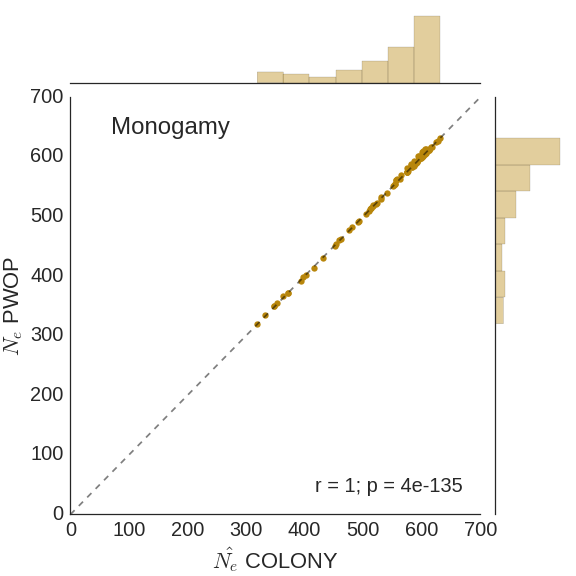
\includegraphics[width=\textwidth]{./Monogamy_mating.png}
\end{figure}

\newpage

\begin{figure}[h!]
	\caption{Scatterplot of $N_e$ estimates with the PWOP and COLONY2 methods for sibling assignments assuming a polygamous mating structure. The Pearson correlation coefficient and p-value (as computed by scipy.stats.pearsonr) are reported.}
	\centering
	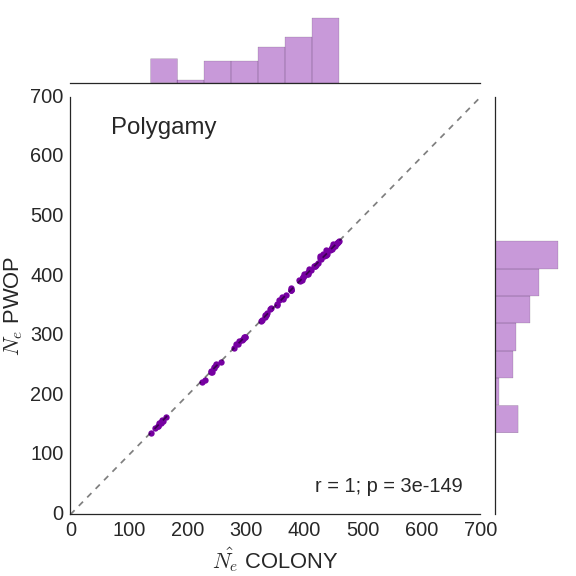
\includegraphics[width=\textwidth]{./Polygamy_mating.png}
\end{figure}

\section*{References}
Crow, James F., and Carter Denniston. "Inbreeding and variance effective population numbers." Evolution (1988): 482-495.

Jones, Owen R., and Jinliang Wang. "COLONY: a program for parentage and sibship inference from multilocus genotype data." Molecular ecology resources 10.3 (2010): 551-555.

Wang, Jinliang. "A new method for estimating effective population sizes from a single sample of multilocus genotypes." Molecular Ecology 18.10 (2009): 2148-2164.

Waples, Robin S., and Ryan K. Waples. "Inbreeding effective population size and parentage analysis without parents." Molecular ecology resources 11.s1 (2011): 162-171.



\end{document}

